\documentclass[11pt]{ainotes}

\title{Fundamentals of Artificial Intelligence and Knowledge Representation\\(Module 2)}
\date{2023 -- 2024}

\begin{document}

    \makenotesfront
    \chapter{Propositional and first order logic}

See \href{https://github.com/NotXia/unibo-ai-notes/tree/pdfs/languages-and-algorithms-for-ai/module2}{\texttt{Languages and Algorithms for AI (module 2)}}.
    \newpage
\lohead{\color{gray} Chapter taken from \href{https://github.com/NotXia/unibo-ai-notes/tree/pdfs/fundamentals-of-ai-and-kr/module2}{\texttt{\color{gray}Fundamentals of AI and KR (module 2)}}}
\lehead{\color{gray} Chapter taken from \href{https://github.com/NotXia/unibo-ai-notes/tree/pdfs/fundamentals-of-ai-and-kr/module2}{\texttt{\color{gray}Fundamentals of AI and KR (module 2)}}}

\graphicspath{{../../fundamentals-of-ai-and-kr/module2/}}
\newpage
\lohead{\color{gray} Chapter taken from \href{https://github.com/NotXia/unibo-ai-notes/tree/pdfs/fundamentals-of-ai-and-kr/module2}{\texttt{\color{gray}Fundamentals of AI and KR (module 2)}}}
\lehead{\color{gray} Chapter taken from \href{https://github.com/NotXia/unibo-ai-notes/tree/pdfs/fundamentals-of-ai-and-kr/module2}{\texttt{\color{gray}Fundamentals of AI and KR (module 2)}}}

\graphicspath{{../../fundamentals-of-ai-and-kr/module2/}}
\newpage
\lohead{\color{gray} Chapter taken from \href{https://github.com/NotXia/unibo-ai-notes/tree/pdfs/fundamentals-of-ai-and-kr/module2}{\texttt{\color{gray}Fundamentals of AI and KR (module 2)}}}
\lehead{\color{gray} Chapter taken from \href{https://github.com/NotXia/unibo-ai-notes/tree/pdfs/fundamentals-of-ai-and-kr/module2}{\texttt{\color{gray}Fundamentals of AI and KR (module 2)}}}

\graphicspath{{../../fundamentals-of-ai-and-kr/module2/}}
\input{../../fundamentals-of-ai-and-kr/module2/sections/_prolog.tex}
\graphicspath{}

\newpage
\lohead{}
\lehead{}
\graphicspath{}

\newpage
\lohead{}
\lehead{}
\graphicspath{}

\newpage
\lohead{}
\lehead{}
    \chapter{Ontologies}

\begin{description}
    \item[Ontology] \marginnote{Ontology} 
        Formal (non-ambiguous) and explicit (obtainable through a finite sound procedure) 
        description of a domain.

    \item[Category] \marginnote{Category}
        Can be organized hierarchically on different levels of generality.

    \item[Object] \marginnote{Object}
        Belongs to one or more categories.

    \item[Upper/general ontology] \marginnote{Upper/general ontology} 
        Ontology focused on the most general domain.

        Properties:
        \begin{itemize}
            \item Should be applicable to almost any special domain.
            \item Combining general concepts should not incur in inconsistences.
        \end{itemize}

        Approaches to create ontologies:
        \begin{itemize}
            \item Created by philosophers/logicians/researchers.
            \item Automatic knowledge extraction from well-structured databases.
            \item Created from text documents (e.g. web).
            \item Crowd-sharing information.
        \end{itemize}
\end{description}


\section{Categories}
\begin{description}
    \item[Category] \marginnote{Category}
        Used in human reasoning when the goal is category-driven (in contrast to specific-instance-driven).

        In first order logic, categories can be represented through:
        \begin{descriptionlist}
            \item[Predicate] \marginnote{Predicate categories}
                A predicate to tell if an object belongs to a category 
                (e.g. \texttt{Car(c1)} indicates that \texttt{c1} is a car).

            \item[Reification] \marginnote{Reification}
                Represent categories as objects as well (e.g. $\texttt{c1} \in \texttt{Car}$).
        \end{descriptionlist}
\end{description}

\subsection{Reification properties and operations}
\begin{description}
    \item[Membership] \marginnote{Membership}
        Indicates if an object belongs to a category.
        (e.g. $\texttt{c1} \in \texttt{Car}$).

    \item[Subclass] \marginnote{Subclass}
        Indicates if a category is a subcategory of another one.
        (e.g. $\texttt{Car} \subset \texttt{Vehicle}$).

    \item[Necessity] \marginnote{Necessity}
        Members of a category enjoy some properties 
        (e.g. $(\text{x} \in \texttt{Car}) \rightarrow \texttt{hasWheels(x)}$).

    \item[Sufficiency] \marginnote{Sufficiency}
        Sufficient conditions to be part of a category\\
        (e.g. $\texttt{hasPlate(x)} \land \texttt{hasWheels(x)} \rightarrow \texttt{x} \in \texttt{Car}$).

    \item[Category-level properties] \marginnote{Category-level properties}
        Category themselves can enjoy properties\\
        (e.g. $\texttt{Car} \in \texttt{VehicleType}$)

    \item[Disjointness] \marginnote{Disjointness}
        Given a set of categories $S$, the categories in $S$ are disjoint iff they all have different objects:
        \[ \texttt{disjoint($S$)} \iff (\forall c_1, c_2 \in S, c_1 \neq c_2 \rightarrow c_1 \cap c_2 = \emptyset) \]

    \item[Exhaustive decomposition] \marginnote{Exhaustive decomposition}
        Given a category $c$ and a set of categories $S$, $S$ is an exhaustive decomposition of $c$ iff
        any element in $c$ belongs to at least a category in $S$:
        \[ \texttt{exhaustiveDecomposition($S$, $c$)} \iff (\forall o \in c \iff \exists c_2 \in S: o \in c_2) \]

    \item[Partition] \marginnote{Partition}
        Given a category $c$ and a set of categories $S$, $S$ is a partition of $c$ when:
        \[ \texttt{partition($S$, $c$)} \iff \texttt{disjoint($S$)} \land \texttt{exhaustiveDecomposition($S$, $c$)} \]
\end{description}


\subsection{Physical composition}
Objects (meronyms) are part of a whole (holonym).

\begin{description}
    \item[Part-of] \marginnote{Part-of}
        If the objects have a structural relation (e.g. $\texttt{partOf(cylinder1, engine1)}$).

        Properties:
        \begin{descriptionlist}
            \item[Transitivity] $\texttt{partOf(x, y)} \land \texttt{partOf(y, z)} \rightarrow \texttt{partOf(x, z)}$
            \item[Reflexivity] $\texttt{partOf(x, x)}$
        \end{descriptionlist}

    \item[Bunch-of] \marginnote{Bunch-of}
        If the objects do not have a structural relation.
        Useful to define a composition of countable objects
        (e.g. $\texttt{bunchOf({nail1, nail3, nail4})}$).
\end{description}


\subsection{Measures}

A property of objects.

\begin{description}
    \item[Quantitative measure] \marginnote{Quantitative measure}
        Something that can be measured using a unit\\
        (e.g. $\texttt{length(table1)} = \texttt{cm(80)}$).

        Qualitative measures propagate when using \texttt{partOf} or \texttt{bunchOf} 
        (e.g. the weight of a car is the sum of its parts).

    \item[Qualitative measure] \marginnote{Qualitative measure}
        Something that can be measured using terms with a partial or total order relation
        (e.g. $\{ \texttt{good}, \texttt{neutral}, \texttt{bad} \}$).

        Qualitative measures do not propagate when using \texttt{partOf} or \texttt{bunchOf}.

    \item[Fuzzy logic] \marginnote{Fuzzy logic}
        Provides a semantics to qualitative measures (i.e. convert qualitative to quantitative).
\end{description}


\subsection{Things vs stuff}

\begin{description}
    \item[Intrinsic property] \marginnote{Intrinsic property}
        Related to the substance of the object. It is retained when the object is divided
        (e.g. water boils at 100°C).

    \item[Extrinsic property] \marginnote{Extrinsic property}
        Related to the structure of the object. It is not retained when the object is divided
        (e.g. the weight of an object changes when split).

    \item[Substance] \marginnote{Substance}
        Category of objects with only intrinsic properties.

        \begin{description}
            \item[Stuff] \marginnote{Stuff}
                The most general substance category.
        \end{description}

    \item[Count noun] \marginnote{Count noun}
        Category of objects with only extrinsic properties.

        \begin{description}
            \item[Things] \marginnote{Things}
                The most general object category.
        \end{description}
\end{description}



\section{Semantic networks}
\marginnote{Semantic networks}
Graphical representation of objects and categories connected through labelled links.

\begin{figure}[h]
    \centering
    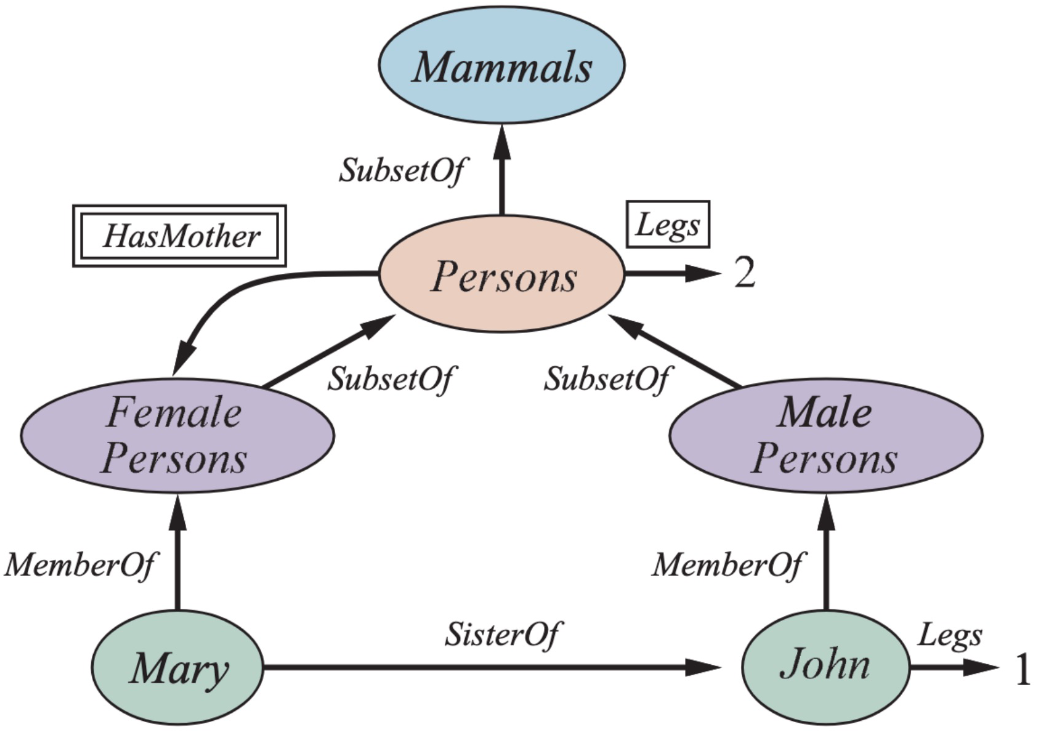
\includegraphics[width=0.4\textwidth]{img/semantic_network.png}
    \caption{Example of semantic network}
\end{figure}

\begin{description}
    \item[Objects and categories] Represented using the same symbol.

    \item[Links] Four different types of links:
        \begin{itemize}
            \item Relation between objects (e.g. \texttt{SisterOf}).
            \item Property of a category (e.g. 2 \texttt{Legs}).
            \item Is-a relation (e.g. \texttt{SubsetOf}).
            \item Property of the members of a category (e.g. \texttt{HasMother}).
        \end{itemize} 
\end{description}

\begin{description}
    \item[Single inheritance reasoning] \marginnote{Single inheritance reasoning}
        Starting from an object, check if it has the queried property.
        If not, iteratively move up to the category it belongs to and check for the property.

    \item[Multiple inheritance reasoning] \marginnote{Multiple inheritance reasoning}
        Reasoning is not possible as it is not clear which parent to choose.
\end{description}

\begin{description}
    \item[Limitations]
        Compared to first order logic, semantic networks do not have:
        \begin{itemize}
            \item Negations.
            \item Universally and existentially quantified properties.
            \item Disjunctions.
            \item Nested function symbols.
        \end{itemize}

        Many semantic network systems allow to attach special procedures to handle special cases 
        that the standard inference algorithm cannot handle.
        This approach is powerful but does not have a corresponding logical meaning.

    \item[Advantages]
        With semantic networks it is easy to attach default properties to categories and
        override them on the objects (i.e. \texttt{Legs} of \texttt{John}).
\end{description}



\section{Frames}
\marginnote{Frames}
Knowledge that describes an object in terms of its properties.
Each frame has:
\begin{itemize}
    \item An unique name
    \item Properties represented as pairs \texttt{<slot - filler>}
\end{itemize}

\begin{example}
    \phantom{}\\[-1em]
    \begin{lstlisting}[mathescape=true, language={}] 
        (
            toronto
                <:Instance-Of City>
                <:Province ontario>
                <:Population 4.5M>
        )
    \end{lstlisting}
\end{example}

\begin{description}
    \item[Prototype] \marginnote{Prototype}
        Members of a category used as comparison metric to determine if another object belongs to the same class
        (i.e. an object belongs to a category if it is similar enough to the prototypes of that category).

    \item[Defeasible value] \marginnote{Defeasible value}
        Value that is allowed to be different when comparing an object to a prototype.

    \item[Facets] \marginnote{Facets}
        Additional information contained in a slot for its filler (e.g. default value, type, domain).

        \begin{description}
            \item[Procedural information] 
                Fillers can be a procedure that can be activated by specific facets:
                \begin{descriptionlist}
                    \item[\texttt{if-needed}] Looks for the value of the slot.
                    \item[\texttt{if-added}] Adds a value.
                    \item[\texttt{if-removed}] Removes a value.
                \end{descriptionlist}
                \begin{example}
                    \phantom{}\\[-1em]
                    \begin{lstlisting}[mathescape=true, language={}] 
    (
        toronto
            <:Instance-Of City>
            <:Province ontario>
            <:Population [if-needed QueryDB]>
    )
                    \end{lstlisting}
                \end{example}
        \end{description}
\end{description}
    \chapter{Description logic}


\section{Syntax}

\begin{description}
    \item[Logical symbols] \marginnote{Logical symbols}
        Symbols with fixed meaning.
        \begin{description}
            \item[Punctuation] ( ) [ ]
            \item[Positive integers] 
            \item[Concept-forming operators] \texttt{ALL}, \texttt{EXISTS}, \texttt{FILLS}, \texttt{AND}
            \item[Connectives] $\sqsubseteq$, $\doteq$, $\rightarrow$
        \end{description}

    \item[Non-logical symbols] \marginnote{Non-logical symbols}
        Domain-dependant symbols.
        \begin{description}
            \item[Atomic concepts] Categories (CamelCase, e.g. \texttt{Person}).
            \item[Roles] Used to describe objects (:CamelCase, e.g. \texttt{:Height}).
            \item[Constants] (camelCase, e.g. \texttt{johnDoe}).
        \end{description}

    \item[Complex concept] \marginnote{Complex concept}
        Concept-forming operators can be used to combine atomic concepts and form complex concepts.
        A well-formed concept follows the conditions:
        \begin{itemize}
            \item An atomic concept is a concept.
            \item If \texttt{r} is a role and \texttt{d} is a concept, then \texttt{[ALL r d]} is a concept.
            \item If \texttt{r} is a role and $n$ is a positive integer, then \texttt{[EXISTS $n$ r]} is a concept.
            \item If \texttt{r} is a role and \texttt{c} is a constant, then \texttt{[FILLS r c]} is a concept.
            \item If $\texttt{d}_1 \dots \texttt{d}_n$ are concepts, 
                then \texttt{[AND $\texttt{d}_1 \dots \texttt{d}_n$]} is a concept.
        \end{itemize}

    \item[Sentence] \marginnote{Sentence}
        Connectives can be used to combine concepts and form sentences.
        A well-formed sentence follows the conditions:
        \begin{itemize}
            \item If $\texttt{d}_1$ and $\texttt{d}_2$ are concepts, 
                then $(\texttt{d}_1 \sqsubseteq \texttt{d}_2)$ is a sentence.
            \item If $\texttt{d}_1$ and $\texttt{d}_2$ are concepts, 
                then $(\texttt{d}_1 \doteq \texttt{d}_2)$ is a sentence.
            \item If $\texttt{c}$ is a constant and $\texttt{d}$ is a concept,
                then $(\texttt{c} \rightarrow \texttt{d})$ is a sentence.
        \end{itemize}

    \item[Knowledge base] \marginnote{Knowledge base}
        Collection of sentences.
        \begin{description}
            \item[Constants] are individuals of the domain.
            \item[Concepts] are categories of individuals.
            \item[Roles] are binary relations between individuals.
        \end{description}


    \item[Assetion box (A-box)] \marginnote{Assetion box (A-box)}
        List of facts about individuals.

    \item[Terminological box (T-box)] \marginnote{Terminological box (T-box)}
        List of sentences (axioms) about concepts.
\end{description}



\section{Semantics}

\subsection{Concept-forming operators}
\marginnote{Concept-forming operators}
Let \texttt{r} be a role, \texttt{d} be a concept, \texttt{c} be a constant and $n$ a positive integer.
The semantics of concept-forming operators are:
\begin{descriptionlist}
    \item[\texttt{[ALL r d]}] 
        Individuals \texttt{r}-related to the individuals of the category \texttt{d}.
        \begin{example}
            \texttt{[ALL :HasChild Male]} individuals that have zero children or only male children.
        \end{example}
    
    \item[\texttt{[EXISTS $n$ r]}] 
        Individuals \texttt{r}-related to at least $n$ other individuals.
        \begin{example}
            \texttt{[EXISTS 1 :Child]} individuals with at least one child.
        \end{example}

    \item[\texttt{[FILLS r c]}] 
        Individuals \texttt{r}-related to the individual \texttt{c}.
        \begin{example}
            \texttt{[FILLS :Child john]} individuals with child \texttt{john}.
        \end{example}

    \item[\texttt{[AND $\texttt{d}_1 \dots \texttt{d}_n$]}] 
        Individuals belonging to all the categories $\texttt{d}_1 \dots \texttt{d}_n$.
\end{descriptionlist}


\subsection{Sentences}
\marginnote{Sentences}
Sentences are expressions with truth values in the domain.
Let \texttt{d} be a concept and \texttt{c} be a constant.
The semantics of sentences are:
\begin{descriptionlist}
    \item[$\texttt{d}_1 \sqsubseteq \texttt{d}_2$]
        Concept $\texttt{d}_1$ is subsumed by $\texttt{d}_2$.
        \begin{example}
            $\texttt{PhDStudent} \sqsubseteq \texttt{Student}$ as every PhD is also a student.
        \end{example}

    \item[$\texttt{d}_1 \doteq \texttt{d}_2$]
        Concept $\texttt{d}_1$ is equivalent to $\texttt{d}_2$.
        \begin{example}
            $\texttt{PhDStudent} \doteq \texttt{[AND Student :Graduated :HasFunding]}$
        \end{example}

    \item[$\texttt{c} \rightarrow \texttt{d}$]
        The individual \texttt{c} satisfies the description of the concept \texttt{d}.
        \begin{example}
            $\texttt{federico} \rightarrow \texttt{Professor}$
        \end{example}
\end{descriptionlist}


\subsection{Interpretation}

\begin{description}
    \item[Interpretation] \marginnote{Interpretation}
        An interpretation $\mathfrak{I}$ in description logic is a pair ($\mathcal{D}, \mathcal{I}$) where:
        \begin{itemize}
            \item $\mathcal{D}$ is the domain.
            \item $\mathcal{I}$ is the interpretation mapping.
                \begin{description}
                    \item[Constant] 
                        Let \texttt{c} be a constant, $\mathcal{I}[\texttt{c}] \in \mathcal{D}$. 
                    \item[Atomic concept] 
                        Let \texttt{a} be an atomic concept, $\mathcal{I}[\texttt{a}] \subseteq \mathcal{D}$. 
                    \item[Role] 
                        Let \texttt{r} be a role, $\mathcal{I}[\texttt{r}] \subseteq \mathcal{D} \times \mathcal{D}$.
                    \item[\texttt{Thing}] 
                        The concept \texttt{Thing} corresponds to the domain: $\mathcal{I}[\texttt{Thing}] = \mathcal{D}$.
                    \item[\texttt{[ALL r d]}]
                        \[
                            \mathcal{I}[\texttt{[ALL r d]}] = 
                            \{ \texttt{x} \in \mathcal{D} \mid \forall \texttt{y}: 
                            \langle \texttt{x}, \texttt{y} \rangle \in \mathcal{I}[r] \text{ then } \texttt{y} \in \mathcal{I}[d] \}
                        \]
                    \item[\texttt{[EXISTS $n$ r]}] 
                        \[ 
                            \mathcal{I}[\texttt{[EXISTS $n$ r]}] = 
                            \{ \texttt{x} \in \mathcal{D} \mid \text{ exists at least $n$ distinct } \texttt{y}: 
                            \langle \texttt{x}, \texttt{y} \rangle \in \mathcal{I}[r] \}
                        \]
                    \item[\texttt{[FILLS r c]}] 
                        \[ 
                            \mathcal{I}[\texttt{[FILLS r c]}] = \{ \texttt{x} \in \mathcal{D} \mid 
                            \langle \texttt{x}, \mathcal{I}[\texttt{c}] \rangle \in \mathcal{I}[\texttt{r}] \} 
                        \]
                    \item[\texttt{[AND $\texttt{d}_1 \dots \texttt{d}_n$]}] 
                        \[ 
                            \mathcal{I}[\texttt{[AND $\texttt{d}_1 \dots \texttt{d}_n$]}] = 
                                \mathcal{I}[\texttt{d}_1] \cap \dots \cap \mathcal{I}[\texttt{d}_n]
                        \]
                \end{description}
        \end{itemize}

    \item[Model] \marginnote{Model}
        Given an interpretation $\mathfrak{I} = (\mathcal{D}, \mathcal{I})$,
        a sentence is true under $\mathfrak{I}$ ($\mathfrak{I} \models \text{sentence}$) if:
        \begin{itemize}
            \item $\mathfrak{I} \models (\texttt{c} \rightarrow \texttt{d})$ iff $\mathcal{I}[\texttt{c}] \in \mathcal{I}[\texttt{d}]$.
            \item $\mathfrak{I} \models (\texttt{d}_\texttt{1} \sqsubseteq \texttt{d}_\texttt{2})$ iff 
                $\mathcal{I}[\texttt{d}_\texttt{1}] \subseteq \mathcal{I}[\texttt{d}_\texttt{2}]$.
            \item $\mathfrak{I} \models (\texttt{d}_\texttt{1} \doteq \texttt{d}_\texttt{2})$ iff 
                $\mathcal{I}[\texttt{d}_\texttt{1}] = \mathcal{I}[\texttt{d}_\texttt{2}]$.
        \end{itemize}

        Given a set of sentences $S$, $\mathfrak{I}$ models $S$ if $\mathfrak{I} \models S$.

    \item[Entailment] \marginnote{Entailment}
        A set of sentences $S$ logically entails a sentence $\alpha$ if:
        \[ \forall \mathfrak{I}:\, (\mathfrak{I} \models S) \rightarrow (\mathfrak{I} \models \alpha) \]
\end{description}



\section{Reasoning}

\subsection{T-box reasoning}

Given a knowledge base of a set of sentences $S$, we would like to be able to determine the following:
\begin{description}
    \item[Satisfiability] \marginnote{Satisfiability}
        A concept \texttt{d} is satisfiable w.r.t. $S$ if:
        \[ \exists \mathfrak{I}, (\mathfrak{I} \models S): \mathfrak{I}[\texttt{d}] \neq \varnothing \]

    \item[Subsumption] \marginnote{Subsumption}
        A concept $\texttt{d}_1$ is subsumed by $\texttt{d}_2$ w.r.t. $S$ if:
        \[ \forall \mathfrak{I}, (\mathfrak{I} \models S): \mathfrak{I}[\texttt{d}_1] \subseteq \mathfrak{I}[\texttt{d}_2] \]

    \item[Equivalence] \marginnote{Equivalence}
        A concept $\texttt{d}_1$ is equivalent to $\texttt{d}_2$ w.r.t. $S$ if:
        \[ \forall \mathfrak{I}, (\mathfrak{I} \models S): \mathfrak{I}[\texttt{d}_1] = \mathfrak{I}[\texttt{d}_2] \]

    \item[Disjointness] \marginnote{Disjointness}
        A concept $\texttt{d}_1$ is disjoint to $\texttt{d}_2$ w.r.t. $S$ if:
        \[ \forall \mathfrak{I}, (\mathfrak{I} \models S): \mathfrak{I}[\texttt{d}_1] \neq \mathfrak{I}[\texttt{d}_2] \]
\end{description}

\begin{theorem}[Reduction to subsumption]
\marginnote{Reduction to subsumption}
    Given the concepts $\texttt{d}_1$ and $\texttt{d}_2$, it holds that:
    \begin{itemize}
        \item $\texttt{d}_1 \text{ is unsatisfiable } \iff \texttt{d}_1 \sqsubseteq \bot$.
        \item $\texttt{d}_1 \doteq \texttt{d}_2 \iff \texttt{d}_1 \sqsubseteq \texttt{d}_2 \land \texttt{d}_2 \sqsubseteq \texttt{d}_1$.
        \item $\texttt{d}_1 \text{ and } \texttt{d}_2 \text{ are disjoint} \iff (\texttt{d}_1 \cap \texttt{d}_2) \sqsubseteq \bot$.
    \end{itemize}
\end{theorem}

\subsection{A-box reasoning}
Given a constant \texttt{c}, a concept \texttt{d} and a set of sentences $S$, we can determine the following:
\begin{description}
    \item[Satisfiability] \marginnote{Satisfiability}
        A constant \texttt{c} satisfies the concept \texttt{d} if:
        \[ S \models (\texttt{c} \rightarrow \texttt{d}) \]

        Note that it can be reduced to subsumption.
\end{description}


\subsection{Computing subsumptions}

Given a knowledge base $KB$ and two concepts \texttt{d} and \texttt{e},
we want to prove:
\[ KB \models (\texttt{d} \sqsubseteq \texttt{e}) \]
The following algorithms can be employed:
\begin{descriptionlist}
    \item[Structural matching] \marginnote{Structural matching}
        \phantom{}
        \begin{enumerate}
            \item Normalize \texttt{d} and \texttt{e} into a conjunctive form:
                \[ \texttt{d} = \texttt{[AND d$_1$ \dots d$_n$]} \hspace*{1cm} \texttt{e} = \texttt{[AND e$_1$ \dots e$_m$]} \]
            \item Check if each part of \texttt{e} is accounted by at least a component of \texttt{d}.
        \end{enumerate}
        
    \item[Tableaux-based algorithms] \marginnote{Tableaux-based algorithms}
        Exploit the following theorem:
        \[ (KB \models (C \sqsubseteq D)) \iff (KB \cup (x : C \sqcap \lnot D)) \text{ is inconsistent} \]

        Note: similar to refutation.
\end{descriptionlist}


\subsection{Open world assumption}

\begin{description}
    \item[Open world assumption] \marginnote{Open world assumption}
        If a sentence cannot be inferred, its truth values is unknown.
\end{description}

Description logics are based on the open world assumption.
To reason in open world assumption, all the possible models are split upon encountering an unknown facts
depending on the possible cases (Oedipus example).



\section{Expanding description logic}
It is possible to expand a description logic by:
\begin{descriptionlist}
    \item[Adding concept-forming operators] \marginnote{Adding concept-forming operators}
        Let \texttt{r} be a role, \texttt{d} be a concept, \texttt{c} be a constant and $n$ a positive integer.
        We can extend our description logic with:
        \begin{description}
            \item[\texttt{[AT-MOST $n$ r]}]
                Individuals \texttt{r}-related to at most $n$ other individuals.
                \begin{example}
                    \texttt{[AT-MOST $1$ :Child]} individuals with only a child.
                \end{example}

            \item[\texttt{[ONE-OF c$_1$ $\dots$ c$_n$]}]
                Concept only satisfied by \texttt{c$_1$ $\dots$ c$_n$}.
                \begin{example}
                    $\texttt{Beatles} \doteq \texttt{[ALL :BandMember [ONE-OF john paul george ringo]]}$
                \end{example}
                
            \item[\texttt{[EXISTS $n$ r d]}]
                Individuals \texttt{r}-related to at least $n$ individuals in the category \texttt{d}.
                \begin{example}
                    \texttt{[EXISTS $2$ :Child Male]} individuals with at least two male children.
                \end{example}
                Note: this increases the computational complexity of entailment.
        \end{description}

    \item[Relating roles] \marginnote{Relating roles}
        \begin{description}
            \item[\texttt{[SAME-AS r$_1$ r$_2$]}]
                Equates fillers of the roles r$_1$ and r$_2$
                \begin{example}
                    \texttt{[SAME-AS :CEO :Owner]}
                \end{example}
                Note: this increases the computational complexity of entailment.
                Role chaining also leads to undecidability.
        \end{description}

    \item[Adding rules] \marginnote{Adding rules}
        Rules are useful to add conditions (e.g. \texttt{if d$_1$ then [FILLS r c]}).
\end{descriptionlist}


\section{Description logics family}

Depending on the number of operators, a description logic can be:
\begin{itemize}
    \item More expressive.
    \item Computationally more expensive.
    \item Undecidable.
\end{itemize}

\begin{description}
    \item[Attributive language ($\mathcal{AL}$)] 
        Minimal description logic with:
        \begin{itemize}
            \item Atomic concepts.
            \item Universal concept (\texttt{Thing} or $\top$).
            \item Bottom concept (\texttt{Nothing} or $\bot$).
            \item Atomic negation (only for atomic concepts).
            \item \texttt{AND} operator ($\sqcap$).
            \item \texttt{ALL} operator ($\forall$).
            \item \texttt{[EXISTS $1$ r]} operator ($\exists$).
        \end{itemize}

    \item[Attributive language complement ($\mathcal{ALC}$)] 
        $\mathcal{AL}$ with negation for concepts.
\end{description}

\begin{table}[h]
    \centering
    \begin{tabular}{|c|c|}
        \hline
        $\mathcal{F}$ & Functional properties \\ \hline
        $\mathcal{E}$ & Full existential quantification \\ \hline
        $\mathcal{U}$ & Concept union \\ \hline
        $\mathcal{C}$ & Complex concept negation \\ \hline
        $\mathcal{S}$ & $\mathcal{ALC}$ with transitive roles \\ \hline
        $\mathcal{H}$ & Role hierarchy \\ \hline
        $\mathcal{R}$ & \makecell[c]{Limited complex roles axioms\\Reflexivity and irreflexivity\\Roles disjointness} \\ \hline
        $\mathcal{O}$ & Nominals \\ \hline
        $\mathcal{I}$ & Inverse properties \\ \hline
        $\mathcal{N}$ & Cardinality restrictions \\ \hline
        $\mathcal{Q}$ & Qualified cardinality restrictions \\ \hline
        $\mathcal{(D)}$ & Datatype properties, data values and data types \\ \hline
    \end{tabular}
    \caption{Name and expressivity of logics}
\end{table}
    \chapter{Web reasoning}


\section{Semantic web}

\begin{description}
    \item[Semantic web] \marginnote{Semantic web}
        Method to represent and reason on the data available on the web.
        Semantic web aims to preserve the characteristics of the web, this includes:
        \begin{itemize}
            \item Globality.
            \item Information distribution.
            \item Information inconsistency of contents and links (as everyone can publish).
            \item Information incompleteness of contents and links.
        \end{itemize}

        Information is structured using ontologies and logic is used as inference mechanism.
        New knowledge can be derived through proofs.

    \item[Uniform resource identifier] \marginnote{URI}
        Naming system to uniquely identify concepts.
        Each URI corresponds to one and only one concept, but multiple URIs can refer to the same concept.

    \item[XML] \marginnote{XML}
        Markup language to represent hierarchically structured data.
        An XML can contain in its preamble the description of the grammar used within the document.

    \item[Resource description framework (RDF)] \marginnote{Resource description framework (RDF)}
        XML-based language to represent knowledge.
        Based on triplets:
        \begin{center}
            \texttt{<subject, predicate, object>}\\
            \texttt{<resource, attribute, value>}
        \end{center}

        RDF supports:
        \begin{descriptionlist}
            \item[Types] Using the attribute \texttt{type} which can assume an URI as value. 
            \item[Collections] Subjects and objects can be bags, sequences or alternatives.
            \item[Meta-sentences] Reification of the sentences (e.g. "X says that Y\dots").
        \end{descriptionlist}

        \begin{description}
            \item[RDF schema] \marginnote{RDF schema}
                RDF can be used to describe classes and relations with other classes (e.g. \texttt{type}, \texttt{subClassOf}, \texttt{subPropertyOf}, \dots)
            
            \item[Representation] \phantom{}
                \begin{descriptionlist}
                    \item[Graph] A graph where nodes are subjects or objects and edges are predicates.
                        \begin{example} \phantom{}
                            \begin{center}
                                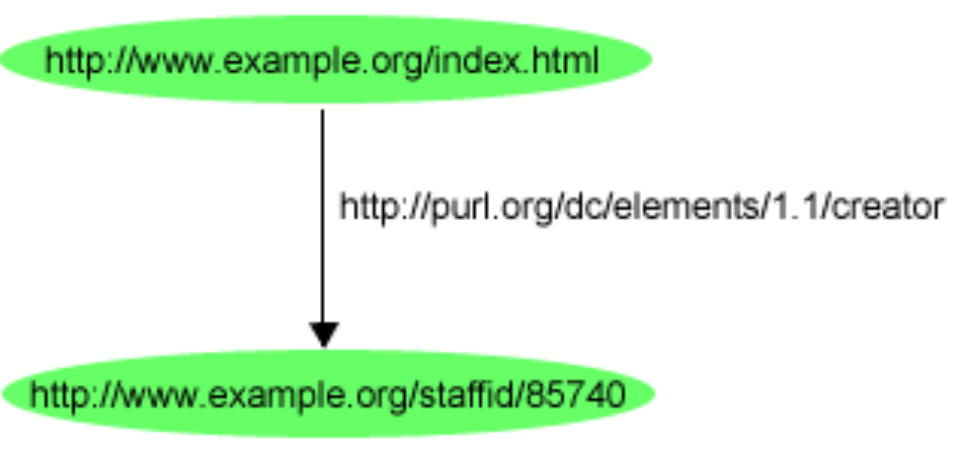
\includegraphics[width=0.4\textwidth]{img/rdf_graph_example.png}
                            \end{center}
                            The graph stands for: 
                            \texttt{http://www.example.org/index.html} has a \texttt{creator} with staff id \texttt{85740}.
                        \end{example}

                    \item[XML]
                        \begin{example} \phantom{}
                            \begin{lstlisting}[mathescape=true, language=xml]
<rdf:RDF
xmlns:rdf=http://www.w3.org/1999/02/22-rdf-syntax-ns#
xmlns:contact=http://www.w3.org/2000/10/swap/pim/contact#>
    <contact:Person rdf:about="http://www.w3.org/People/EM/contact#me">
        <contact:fullName>Eric Miller</contact:fullName>
        <contact:mailbox rdf:resource="mailto:em@w3.org"/>
        <contact:personalTitle>Dr.</contact:personalTitle>
    </contact:Person>
</rdf:RDF>
                            \end{lstlisting}
                        \end{example}
                \end{descriptionlist}

            \item[Database similarities]
                RDF aims to integrate different databases:
                \begin{itemize}
                    \item A DB record is an RDF node.
                    \item The name of a column can be seen as a property type.
                    \item The value of a field corresponds to the value of a property.
                \end{itemize}
        \end{description}

    \item[RDFa] \marginnote{RDFa}
        Specification to integrate XHTML and RDF.

    \item[SPARQL] \marginnote{SPARQL}
        Language to query different data sources that support RDF (natively or through a middleware).

    \item[Ontology web language (OWL)] \marginnote{Ontology web language (OWL)}
        Ontology-based on RDF and description logic fragments.
        Three levels of expressivity are available:
        \begin{itemize}
            \item OWL lite.
            \item OWL DL.
            \item OWL full.
        \end{itemize}

        An OWL has:
        \begin{descriptionlist}
            \item[Classes] Categories.
            \item[Properties] Roles and relations.
            \item[Instances] Individuals.
        \end{descriptionlist}
\end{description}



\section{Knowledge graphs}

\begin{description}
    \item[Knowledge graph] \marginnote{Knowledge graph}
        Knowledge graphs overcome the computational complexity of T-box reasoning with semantic web and description logics.

        \begin{itemize}
            \item Use a simple vocabulary with a simple but robust corpus of types and properties adopted as a standard.
            \item Represent a graph with terms as nodes and edges connecting them.
                Knowledge is therefore represented as triplets \texttt{(h, r, t)} where \texttt{h} and \texttt{t} are entities and \texttt{r} is a relation.
            \item Logic formulas are removed. T-box and A-box can be seen as the same concept. There is no reasoning but only facts.
            \item Data does not have a conceptual schema and can come from different sources with different semantics.
            \item Graph algorithms to traverse the graph and solve queries.
        \end{itemize}

    \item[KG quality] \marginnote{Quality}
        \begin{description}
            \item[Coverage] If the graph has all the required information.
            \item[Correctness] If the information is correct (can be objective or subjective).
            \item[Freshness] If the content is up-to-date.
        \end{description}

    \item[Graph embedding] \marginnote{Graph embedding}
        Project entities and relations into a vectorial space for ML applications.
        \begin{description}
            \item[Entity prediction] Given two entities \texttt{h} and \texttt{t}, determine the relation \texttt{r} between them.
            \item[Link prediction] Given an entity \texttt{h} and a relation \texttt{t}, determine an entity \texttt{t} related to \texttt{h}.
        \end{description}
\end{description}
    \chapter{Time reasoning}


\section{Propositional logic}

\begin{description}
    \item[State] \marginnote{State} 
        The current state of the world can be represented as a set of propositions that are true according to the observation of an agent.

        The union of a countable sequence of states represents the evolution of the world. Each proposition is distinguished by its time step.

        \begin{example}
            A child has a bow and an arrow and then shoots the arrow.
            \[
                \begin{split}
                    \text{KB}^0 &= \{ \texttt{hasBow}^0, \texttt{hasArrow}^0  \} \\
                    \text{KB}^1 &= \{ \texttt{hasBow}^0, \texttt{hasArrow}^0, \texttt{hasBow}^1, \lnot\texttt{hasArrow}^1  \} 
                \end{split}
            \]
        \end{example}

    \item[Action] \marginnote{Action}
        An action indicates how a state evolves into the next one.
        It is described using effect axioms in the form:
        \[ \texttt{action}^t \Rightarrow (\texttt{preconditions}^t \iff \texttt{effects}^{t+1}) \]

        \begin{description}
            \item[Frame problem] \marginnote{Frame problem}
                The effect axioms of an action do not tell what remains unchanged in the next state.

            \begin{description}
                \item[Frame axioms] \marginnote{Frame axioms}
                    The frame axioms of an action describe the unaffected propositions of an action.
            \end{description}
        \end{description}

        \begin{example}
            The action of shooting an arrow can be described as:
            \[
                \begin{split}
                    \texttt{SHOOT}^t &\Rightarrow \{ \texttt{hasArrow}^t \iff \lnot\texttt{hasArrow}^{t+1} \} \\
                    \texttt{SHOOT}^t &\Rightarrow \{ \texttt{hasBow}^t \iff \texttt{hasBow}^{t+1} \}
                \end{split}  
            \]
        \end{example}

        Note that with $m$ actions and $n$ propositions, the number of frame axioms will be of order $O(mn)$.
        Inference for $t$ time steps will have complexity $O(nt)$.
\end{description}



\section{Situation calculus (Green's formulation)}
Situation calculus uses first-order logic instead of propositional logic.

\begin{description}
    \item[Situation] \marginnote{Situation}
        The initial state is a situation.
        Applying an action in a situation is a situation:
        \[ s \text{ is a situation and } \texttt{a} \text{ is an action} \iff \texttt{result}(\texttt{a}, s) \text{ is situation} \]
        (Note: in FAIRK module 1, \texttt{result} is denoted as \texttt{do}).

    \item[Fluent] \marginnote{Fluent}
        Function that varies depending on the situation 
        (i.e. tells if a property holds in a given situation).

        \begin{example}
            $\texttt{hasBow}(s)$ where $s$ is a situation.
        \end{example}

    \item[Action] \marginnote{Action}
        Actions are described using:
        \begin{descriptionlist}
            \item[Possibility axioms] \marginnote{Possibility axioms}
                Indicates the preconditions $\phi_\texttt{a}$ of an action \texttt{a} in a given situation $s$:
                \[ \phi_\texttt{a}(s) \Rightarrow \texttt{poss}(\texttt{a}, s) \]

            \item[Successor state axiom] \marginnote{Successor state axiom}
                The evolution of a fluent $F$ follows the axiom:
                \[ F^{t+1} \iff (\texttt{ActionCauses$(F)$} \vee (F^{t} \land \lnot\texttt{ActionCauses$(\lnot F)$})) \]
                In other words, a fluent is true if an action makes it true or does not change if the action does not involve it.

                Adding the notion of possibility, an action can be described as:
                \[ 
                    \begin{split}
                        \texttt{poss}&(\texttt{a}, s) \Rightarrow \Big( F(\texttt{result}(\texttt{a}, s)) \iff \\
                            & (\texttt{a} = \texttt{ActionCauses$(F)$}) \,\vee\, \\
                            & (F(s) \,\land\, \texttt{a} \neq \lnot\texttt{ActionCauses$(\lnot F)$})
                        \Big)
                    \end{split}
                \]
            
            \item[Unique action axiom] \marginnote{Unique action axiom}
                Only a single action can be executed in a situation to avoid non-determinism.
        \end{descriptionlist}
\end{description}



\section{Event calculus (Kowalski's formulation)}

Event calculus reifies fluents and events (actions) as terms (instead of predicates).

\begin{description}
    \item[Event calculus ontology] \marginnote{Event calculus ontology}
        A fixed set of predicates:
        \begin{descriptionlist}
            \item[$\texttt{holdsAt}(F, T)$] The fluent $F$ holds at time $T$.
            \item[$\texttt{happens}(\texttt{E}, T)$] The event \texttt{E} (i.e. execution of an action) happened at time $T$.
            \item[$\texttt{initiates}(\texttt{E}, F, T)$] The event \texttt{E} causes the fluent $F$ to start holding at time $T$.
            \item[$\texttt{terminates}(\texttt{E}, F, T)$] The event \texttt{E} causes the fluent $F$ to cease holding at time $T$.
            \item[$\texttt{clipped}(T_i, F, T_j)$] The fluent $F$ has been made false between the times $T_i$ and $T_j$ ($T_i < T_j$).
            \item[$\texttt{initially}(F)$] The fluent $F$ holds at time 0.
        \end{descriptionlist}

    \item[Domain-independent axioms] \marginnote{Domain-independent axioms}
        A fixed set of axioms:
        \begin{description}
            \item[Truthness of a fluent] \phantom{}
                \begin{enumerate}
                    \item A fluent holds if an event initiated it in the past and has not been clipped.
                        \[ 
                            \begin{split}
                                \texttt{holdsAt}(F, T_j) \Leftarrow\, &\texttt{happens}(\texttt{E}, T_i) \land (T_i < T_j) \,\land\\
                                    &\texttt{initiates}(\texttt{E}, F, T_i) \land \lnot\texttt{clipped}(T_i, F, T_j)
                            \end{split}
                        \]

                    \item A fluent holds if it was initially true and has not been clipped.
                        \[ \texttt{holdsAt}(F, T) \Leftarrow\, \texttt{initially}(F) \land \lnot\texttt{clipped}(0, F, T) \]
                \end{enumerate}
                Note: the negations make the definition of these axioms in Prolog unsafe.
            
            \item[Clipping of a fluent]
                \[ \texttt{clipped}(T_i, F, T_j) \Leftarrow \texttt{happens}(\texttt{E}, T) \land (T_i < T < T_j) \land \texttt{terminates}(\texttt{E}, F, T) \]
        \end{description}

    \item[Domain-dependent axioms] \marginnote{Domain-dependent axioms}
        Domain-specific axioms defined using the predicates\\\texttt{initially}, \texttt{initiates} and \texttt{terminates}.
\end{description}

\begin{description}
    \item[Deductive reasoning] 
        Event calculus only allows deductive reasoning: 
        it takes as input the domain-dependant axioms and a set of events and computes a set of true fluents.
        If a new event is observed, the query needs to be recomputed again.
\end{description}


\begin{example}
    A room with a light and a button can be described as:
    \begin{descriptionlist}
        \item[Fluents] \texttt{lightOn} $\cdot$ \texttt{lightOff}
        \item[Events] \texttt{PUSH\_BUTTON}
    \end{descriptionlist}

    Domain-dependent axioms are:
    \begin{descriptionlist}
        \item[Initial state] \texttt{initially}(\texttt{lightOff}) 
        \item[Effects of \texttt{PUSH\_BUTTON} on \texttt{lightOn}] \phantom{}
            \begin{itemize}
                \item $\texttt{initiates}(\texttt{PUSH\_BUTTON}, \texttt{lightOn}, T) \Leftarrow \texttt{holdsAt}(\texttt{lightOff}, T)$
                \item $\texttt{terminates}(\texttt{PUSH\_BUTTON}, \texttt{lightOn}, T) \Leftarrow \texttt{holdsAt}(\texttt{lightOn}, T)$
            \end{itemize}
        \item[Effects of \texttt{PUSH\_BUTTON} on \texttt{lightOff}] \phantom{}
            \begin{itemize}
                \item $\texttt{initiates}(\texttt{PUSH\_BUTTON}, \texttt{lightOff}, T) \Leftarrow \texttt{holdsAt}(\texttt{lightOn}, T)$
                \item $\texttt{terminates}(\texttt{PUSH\_BUTTON}, \texttt{lightOff}, T) \Leftarrow \texttt{holdsAt}(\texttt{lightOff}, T)$
            \end{itemize}
    \end{descriptionlist}

    A set of events could be:
    \[ \texttt{happens}(\texttt{PUSH\_BUTTON}, 3) \cdot \texttt{happens}(\texttt{PUSH\_BUTTON}, 5) \cdot \texttt{happens}(\texttt{PUSH\_BUTTON}, 6) \]
\end{example}


\subsection{Reactive event calculus}
\marginnote{Reactive event calculus}

Allows to add events dynamically without the need to recompute the result.



\section{Allen's logic of intervals}

Event calculus only captures instantaneous events that happen at given points in time.

\begin{description}
    \item[Allen's logic of intervals] \marginnote{Allen's logic of intervals}
        Reasoning on time intervals.

        \begin{description}
            \item[Interval] \marginnote{Interval} 
                An interval $i$ starts at a time $\texttt{begin}(i)$ and ends at a time $\texttt{end}(i)$.

            \item[Temporal operators] \marginnote{Temporal operators}
                \begin{itemize}
                    \item $\texttt{meet}(i, j) \iff \texttt{end}(i) = \texttt{begin}(j)$
                    \item $\texttt{before}(i, j) \iff \texttt{end}(i) < \texttt{begin}(j)$
                    \item $\texttt{after}(i, j) \iff \texttt{before}(j, i)$
                    \item $\texttt{during}(i, j) \iff \texttt{begin}(j) < \texttt{begin}(i) < \texttt{end}(i) < \texttt{end}(j)$
                    \item $\texttt{overlap}(i, j) \iff \texttt{begin}(i) < \texttt{begin}(j) < \texttt{end}(i) < \texttt{end}(j)$
                    \item $\texttt{starts}(i, j) \iff \texttt{begin}(i) = \texttt{begin}(j)$
                    \item $\texttt{finishes}(i, j) \iff \texttt{end}(i) = \texttt{end}(j)$
                    \item $\texttt{equals}(i, j) \iff \texttt{starts}(i, j) \land \texttt{ends}(i, j)$
                \end{itemize}

                \begin{figure}[H]
                    \centering
                    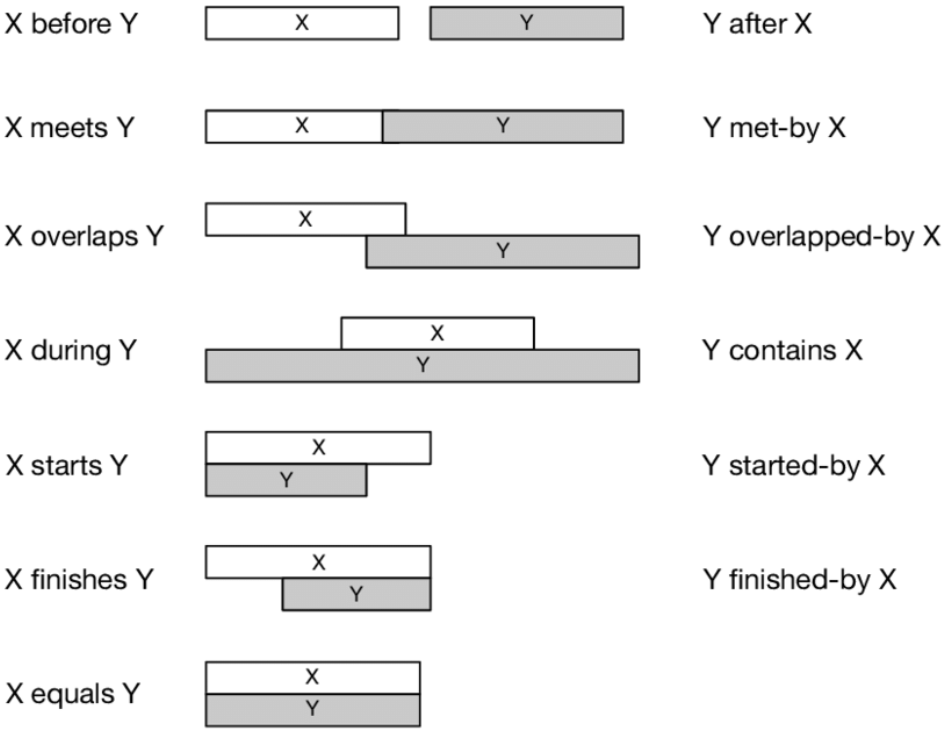
\includegraphics[width=0.5\textwidth]{img/allen_intervals.png}
                    \caption{Visual representation of temporal operators}
                \end{figure}
        \end{description}
\end{description}



\section{Modal logics}

Logic-based on interacting agents with their own knowledge base.

\begin{description}
    \item[Propositional attitudes] \marginnote{Propositional attitudes}
        Operators to represent knowledge and beliefs of an agent towards the environment and other agents.

        First-order logic is not suited to represent these operators.

    \item[Modal logics] \marginnote{Modal logics}
        Modal logics have the same syntax as first-order logic with the addition of modal operators.

    \item[Modal operator]
        A modal operator takes as input the name of an agent and a sentence (instead of a term as in FOL).
        
        \begin{description}
            \item[Knowledge operator] \marginnote{Knowledge operator}
                Operator to indicate that an agent \texttt{a} knows $P$:
                \[ \textbf{K}_\texttt{a}(P) \]

            \item[Belief operator]
            \item[Everyone knows operator]
            \item[Common knowledge operator]
            \item[Distribute knowledge operator]
        \end{description}

        Depending on the operators, different modal logics can be defined.

    \item[Semantics]
        An agent has a current perception of the world and considers the unknown as other possible worlds.
        Moreover, if $P$ is true in any accessible world from the current one, the agent has knowledge of $P$.

        Formally, semantics is defined on a set of primitive propositions $\phi$ 
        using a Kripke structure $M = (S, \pi, K_\texttt{1}, \dots, K_\texttt{n})$ where:
        \begin{itemize}
            \item $S$ is a set of the states of the world.
            \item $\pi: \phi \rightarrow 2^S$ specifies in which states each primitive proposition holds.
            \item $K_\texttt{i} \subseteq S \times S$ is a binary relation where 
                $(s, t) \in K_\texttt{i}$ if an agent \texttt{i} considers the world $t$ possible (accessible) from $s$.
                In other words, when the agent is in the world $s$, it considers $t$ to also be a possibly valid world.
                Obviously, $(s, s) \in K_\texttt{i}$ for all states.
        \end{itemize}

        \begin{example}
            Alice is in a room and tosses a coin. Bob is in another room and will enter Alice's room when the coin lands to observe the result.

            We define a model $M = (S, \pi, K_\texttt{a}, K_\texttt{b})$ on $\phi$ where:
            \begin{itemize}
                \item $\phi = \{ \texttt{tossed}, \texttt{heads}, \texttt{tails} \}$.
                \item $S = \{ s_0, h_1, t_1, h_2, t_2 \}$ where the possible states are divided in three stages:
                    the initial state ($s_0$), the result of the coin flip ($h_1, t_1$) and the observation of Bob ($h_2, t_2$).
                \item 
                    $\pi(\texttt{tossed}) = \{ h_1, t_1, h_2, t_2 \}$\\
                    $\pi(\texttt{heads}) = \{ h_1, h_2 \}$\\
                    $\pi(\texttt{tails}) = \{ t_1, t_2 \}$
                \item 
                    $K_\texttt{a} = \{ (s, s) \mid s \in S \}$ as Alice observes everything in each world and does not have uncertainty.\\
                    $K_\texttt{b} = \{ (s, s) \mid s \in S \} \cup \{ (h_1, t_1), (t_1, h_1) \}$ as Bob is unsure of what happens in the second stage.\\
            \end{itemize}
            \vspace*{-1em}
            With this model, we can determine the truthness of sentences like:
            \[ (M, s_0) \models K_\texttt{a}(\lnot\texttt{tossed}) \land K_\texttt{b}\Big(K_\texttt{a}\big(K_\texttt{b}(\lnot \texttt{heads} \land \lnot \texttt{tails})\big)\Big) \]
            \[ (M, t_1) \models (\texttt{heads} \vee \texttt{tails}) \land \lnot\texttt{K}_\texttt{b}(\texttt{heads}) \land 
                \lnot\texttt{K}_\texttt{b}(\texttt{tails}) \land 
                \texttt{K}_\texttt{b}(\texttt{K}_\texttt{a}(\texttt{heads}) \vee \texttt{K}_\texttt{a}(\texttt{tails})) \]
        \end{example}
    
    \item[Axioms] \phantom{}
        \begin{description}
            \item[Tautology] 
                All propositional tautologies are valid.

            \item[Modus ponens] 
                If $\varphi$ and $\varphi \Rightarrow \psi$ are valid, then $\psi$ is valid.

            \item[Distribution axiom] 
                Knowledge is closed under implication:
                \[ (K_\texttt{i}(\varphi) \land K_\texttt{i}(\varphi \Rightarrow \psi)) \Rightarrow K_\texttt{i}(\psi) \]

            \item[Knowledge generalization rule] 
                An agent knows all the tautologies:
                \[ \forall \text{ structures } M: (M \models \varphi) \Rightarrow (M \models K_\texttt{i}(\varphi)) \]

            \item[Knowledge axiom] 
                If an agent knows $\varphi$, then $\varphi$ is true:
                \[ K_\texttt{i}(\varphi) \Rightarrow \varphi \]

                In belief logic, this axiom is substituted with $\lnot K_\texttt{i}(\texttt{false})$.

            \item[Introspection axioms]
                An agent is sure of its knowledge:
                \begin{description}
                    \item[Positive] $K_\texttt{i}(\varphi) \Rightarrow K_\texttt{i}(K_\texttt{i}(\varphi))$ 
                    \item[Negative] $\lnot K_\texttt{i}(\varphi) \Rightarrow K_\texttt{i}(\lnot K_\texttt{i}(\varphi))$ 
                \end{description}
        \end{description}
        
        Different modal logics can be defined based on the validity of these axioms.
\end{description}



\section{Temporal logics}

Logics based on modal logic with the addition of a temporal dimension.
Time is discrete and each world is labeled with an integer. 
The accessibility relation maps into the temporal dimension with two possible evolution alternatives:
\begin{descriptionlist}
    \item[Linear-time] \marginnote{Linear-time}
        From each world, there is only one other accessible world.
    
    \item[Branching-time] \marginnote{Branching-time}
        From each world, there are many accessible worlds.
\end{descriptionlist}




\subsection{Linear-time temporal logic}

\begin{description}
    \item[Operators] \phantom{}
        \begin{description}
            \item[Next ($\bigcirc \varphi$)] \marginnote{Next}
                $\varphi$ is true in the next time step.

            \item[Globally ($\square \varphi$)] \marginnote{Globally}
                $\varphi$ is always true from now on.

            \item[Future ($\diamond \varphi$)] \marginnote{Future}
                $\varphi$ is sometimes true in the future.
                It is equivalent to $\lnot\square(\lnot \varphi)$.

            \item[Until ($\varphi \mathcal{U} \psi$)] \marginnote{Until}
                There exists a moment (now or in the future) when $\psi$ holds. 
                $\varphi$ is guaranteed to hold from now until $\psi$ starts to hold.

            \item[Weak until ($\varphi \mathcal{W} \psi$)] \marginnote{Weak until}
                There might be a moment when $\psi$ holds. 
                $\varphi$ is guaranteed to hold from now until $\psi$ possibly starts to hold.
        \end{description}

    \item[Semantics]
        Given a Kripke structure, $M = (S, \pi, K_\texttt{1}, \dots, K_\texttt{n})$ where states are represented using integers,
        the semantics of the operators is the following:
        \begin{itemize}
            \item $(M, i) \models P \iff i \in \pi(P)$.
            \item $(M, i) \models \bigcirc\varphi \iff (M, i+1) \models \varphi$.
            \item $(M, i) \models \square\varphi \iff \forall j \geq i: (M, j) \models \varphi$.
            \item $(M, i) \models \varphi \mathcal{U} \psi \iff \exists k \geq i: \big( (M, k) \models \psi \,\land\, \forall j. i \leq j \leq k: (M, j) \models \varphi \big)$.
            \item $(M, i) \models \varphi \mathcal{W} \psi \iff ((M, i) \models \varphi \mathcal{U} \psi) \vee ((M, i) \models \square\varphi)$.
        \end{itemize}

    \item[Model checking] \marginnote{Model checking}
        Methods to prove properties of linear-time temporal logic-based finite state machines or distributed systems.
\end{description}
    \chapter{Probabilistic logic reasoning}

\begin{description}
    \item[Probabilistic logic programming] \marginnote{Probabilistic logic programming}
        Adds probability distributions over logic programs allowing to define different worlds.
        Joint distributions can also be defined over worlds and allow to answer to queries.
\end{description}



\section{Logic programs with annotated disjunctions (LPAD)}
\marginnote{LPAD}

\subsection{Syntax}

\begin{description}
    \item[\texttt{null}] 
        Atom that can only appear in the head of a clause and 
        cancels the clause (i.e. equivalent of not having the clause).
\end{description}

The head of each clause is defined as a disjunction of atoms, each with a probability.
More specifically, each clause has a probability distribution over its head.

\begin{example}
    \phantom{}
    \begin{lstlisting}
    sneezing(X):0.7 ; null:0.3 :- flu(X).
    sneezing(X):0.8 ; null:0.2 :- hay_fever(X).
    \end{lstlisting}
\end{example}


\subsection{Distribution semantics}

\begin{description}
    \item[Worlds] \marginnote{World}
        Given a clause $C$ and a substitution $\theta$ such that $C\theta$ is ground,
        the following operations are defined for LPAD:
        \begin{descriptionlist}
            \item[Atomic choice] \marginnote{Atomic choice}
                An atomic choice $(C, \theta, i)$ is the selection of the $i$-th atom in the head of $C$ for grounding.

            \item[Composite choice] \marginnote{Composite choice}
                A composite choice $\kappa$ is a set of atomic choices.
                The probability of a composite choice is the following:
                \[ \prob{\kappa} = \prod_{(C, \theta, i) \in \kappa} \prob{C, i} \]
                where $\prob{C, i}$ is the probability of choosing the $i$-th atom in the head of $C$.

            \item[Selection] \marginnote{Selection}
                A selection $\sigma$ is a composite choice where an atom from the head of each clause for each grounding has been chosen.
                In other words, a selection can be defined only when the program is ground.

                A selection $\sigma$ identifies a world $w_\sigma$ and has probability:
                \[ \prob{w_\sigma} = \prob{\sigma} = \prod_{(C, \theta, i) \in \sigma} \prob{C, i} \]
        \end{descriptionlist}

        \begin{example}
            Given the program:
            \begin{lstlisting}
    sneezing(X):0.7 ; null:0.3 :- flu(X).
    sneezing(X):0.8 ; null:0.2 :- hay_fever(X).
            \end{lstlisting}

            The possible worlds are:
            \begin{center}
                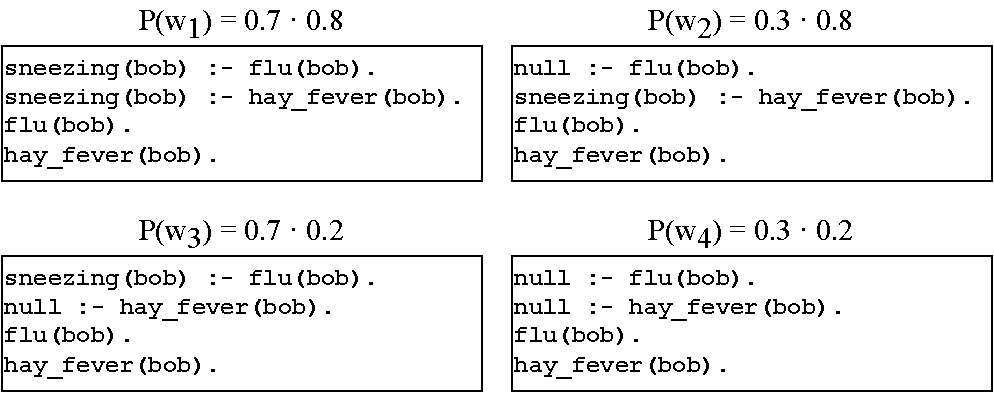
\includegraphics[width=0.7\textwidth]{img/_probabilistic_logic_example.pdf}
            \end{center}
        \end{example}

    \item[Queries] \marginnote{Queries}
        Given a ground query $Q$ and a world $w$, the probability of $Q$ being true in $w$ is trivially:
        \[ 
            \prob{Q \mid w}
            \begin{cases}
                1 & \text{ if $Q$ is true in $w$}\\
                0 & \text{ otherwise}
            \end{cases} 
        \]

        The overall probability of $Q$ is:
        \[ \prob{Q} = \sum_w \prob{Q, w} = \sum_w \prob{Q \mid w}\prob{w} = \sum_{w \models Q} \prob{w} \]

        \begin{example}
            Given the program:
            \begin{lstlisting}
    sneezing(X):0.7 ; null:0.3 :- flu(X).
    sneezing(X):0.8 ; null:0.2 :- hay_fever(X).
            \end{lstlisting}

            The probability of \texttt{sneezing(bob)} is:
            \[ \prob{\texttt{sneezing(bob)}} = \prob{w_1} + \prob{w_2} + \prob{w_3} \]
        \end{example}
\end{description}
    \chapter{Forward reasoning}

\begin{description}
    \item[Logical implication] \marginnote{Logical implication}
        Simplest form of rule:
        \[ p_1, \dots, p_n \Rightarrow q_1, \dots, q_m \]
        where:
        \begin{descriptionlist}
            \item[Left hand side (LHS)] $p_1, \dots, p_n$
            \item[Right hand side (RHS)] $q_1, \dots, q_m$
        \end{descriptionlist}
    
    \item[Modus ponens] \marginnote{Modus ponens}
        If $A$ and $A \Rightarrow B$ are true, then we can derive that $B$ is true.

    \item[Production rules] \marginnote{Production rules}
        Approach that allows to dynamically add facts to the knowledge base (differently from backward reasoning in Prolog).

        When a fact is added, the reasoning mechanism is triggered:
        \begin{descriptionlist}
            \item[Match] Search for the rules whose LHS match the fact and (arbitrarily) decide which to trigger.
            \item[Conflict resolution] Triggered rules are put in an agenda where conflicts are solved.
            \item[Execution] The RHS of the triggered rules are executed and the effects are performed.
                The knowledge base is updated with the (copies of the) new facts.
        \end{descriptionlist}
        These steps are executed until quiescence as the execution step may add new facts.

    \item[Working memory] \marginnote{Working memory}
        Data structure that contains the currently valid set of facts and rules.

        The performance of a production rules system depends on the efficiency of the working memory.
\end{description}



\section{RETE algorithm}

RETE is an efficient algorithm for implementing rule-based systems.

\subsection{Match}
\begin{description}
    \item[Pattern] \marginnote{Pattern}
        The LHS of a rule is expressed as a conjunction of patterns (conditions).

        A pattern can test:
        \begin{descriptionlist}
            \item[Intra-element features] Features that can be tested directly on a fact.
            \item[Inter-element features] Features that involve more facts.
        \end{descriptionlist}

    \item[Conflict set] \marginnote{Conflict set}
        Set of all possible instantiations of production rules.
        Each rule is described as:
        \[ \langle \text{Rule}, \text{ list of facts matched by its LHS} \rangle \]

        Instead of naively checking a rule over all the facts, each rule has associated the facts that match its LHS patterns.

    \item[LHS network]
        Compile the LHSs into networks:
        \begin{descriptionlist}
            \item[Alpha-network] \marginnote{Alpha-network}
                For intra-element features.
                The outcome is stored in alpha-memories and used by the beta network.

            \item[Beta-network] \marginnote{Beta-network}
                For inter-element features.
                The outcome is stored in beta-memories and corresponds to the conflict set.
        \end{descriptionlist}
        If more rules use the same pattern, the node of that pattern is reused and possibly outputting to different memories.
\end{description}


\subsection{Conflict resolution}
RETE allows different strategies to handle conflicts:
\begin{itemize}
    \item Rule priority.
    \item Rule ordering.
    \item Temporal attributes.
    \item Rule complexity.
\end{itemize}
The best approach depends on the use case.


\subsection{Execution}
By default, RETE executes all the rules in the agenda and 
then checks for possible side effects that modify the working memory in a second moment.

Note that it is very easy to create loops.



\section{Drools framework}
\marginnote{Drools}

RETE-based rule engine that uses Java.

\begin{description}
    \item[Rule] A rule has structure:
        \begin{lstlisting}[language={java}]
            rule "rule name"
                // Rule attributes
            when
                // LHS
            then
                // RHS
            end
        \end{lstlisting}

    \item[Quantifiers] \phantom{}
        \begin{description}
            \item[\texttt{exists P(...)}] 
                Trigger the rule once if at least a fact \texttt{P(...)} exists in the working memory. 
            \item[\texttt{forall P(...)}] 
                Trigger the rule if all the instances of \texttt{P(...)} match.
                The rule can be executed multiple times. 
            \item[\texttt{not P(...)}] 
                Trigger the rule if the fact \texttt{P(...)} does not exist in the working memory. 
                Note that a negation in different positions might result in different behaviors.
        \end{description}

    \item[Consequences] 
        Drools allows two types of RHS operations:
        \begin{description}
            \item[Logic] \phantom{}
                \begin{description}
                    \item[Insert] 
                        Create a new fact and insert it in the working memory.
                        Existing rules may trigger if they match the new fact.

                        If the conditions of the rule that inserted a fact are no longer true, the inserted fact is automatically retracted.

                    \item[Retract]  Remove a fact from the working memory.
                    
                    \item[Modify] 
                        A combination of retract and insert executed consecutively.
                        The \texttt{no-loop} keyword can be used to avoid loops.
                \end{description}

            \item[Non-logic]
                Execution of Java code or external side effects.
        \end{description}

    \item[Conflict resolution] \phantom{}
        \begin{description}
            \item[Salience score]
            \item[Agenda group]
                Associate a group to each rule. The method \texttt{setFocus} can be used to prioritize certain groups.
            \item[Activation group]
                Only one rule among the ones with the same activation group is executed (i.e. mutual exclusion).
        \end{description}
\end{description}



\section{Complex event processing}

\begin{description}
    \item[Event] \marginnote{Event}
        Information with a description and temporal information (instantaneous or with a duration).

    \item[Simple event] \marginnote{Simple event}
        Event detected outside an event processing system (e.g. a sensor). It does not provide any information alone.

    \item[Complex event] \marginnote{Complex event}
        Event generated by an event processing system and able to provides a higher informative payload.

    \item[Complex event processing (CEP)] \marginnote{Complex event processing}
        Paradigm for dealing with a large amount of information.
        Takes as input different types of events and outputs durative events.
\end{description}


\subsection{Drools}

Drools supports CEP by representing events as facts.

\begin{description}
    \item[Clock]
        Mechanism to specify time conditions to reason over temporal intervals.

    \item[Sliding windows] \phantom{}
        \begin{description} 
            \item[Time-based window] Select events within a time slice. 
            \item[Length-based window] Select the last $n$ events.
        \end{description}

    \item[Expiration]
        Mechanism to specify an expiration time for events and discard them from the working memory.

    \item[Temporal reasoning]
        Allen's temporal operators for temporal reasoning.
\end{description}

\end{document}